\section{Results}
\subsection{Minikube results}
After running the commands in Listings~\ref{lst:minikube-cluster}, the Minikube creates a three-node cluster with two worker nodes and one control plane node.
This is shown in Figure~\ref{fig:minikube-cluster}.

\begin{figure}[!htbp]
  \centering
  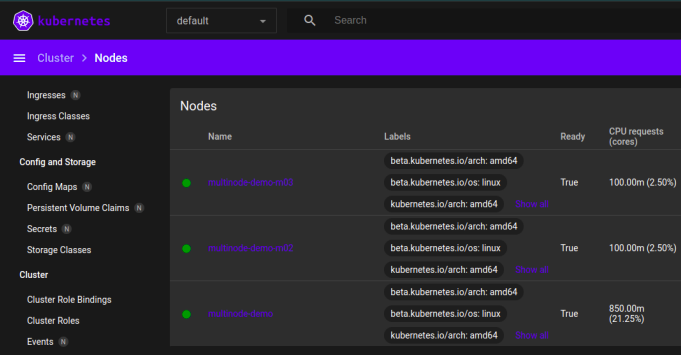
\includegraphics[width=0.45\textwidth]{figures/nodes.png}
  \caption{Minikube cluster with three nodes.}
  \label{fig:minikube-cluster}
\end{figure}

After running the commands in Listings~\ref{lst:kubectl_php_apache}, the PHP Apache server is deployed on the Minikube cluster.
The dashboard shows the deployment and service created, as shown in Figure~\ref{fig:deployments} and Figure~\ref{fig:services}, respectively.

\begin{figure}[!htbp]
  \centering
  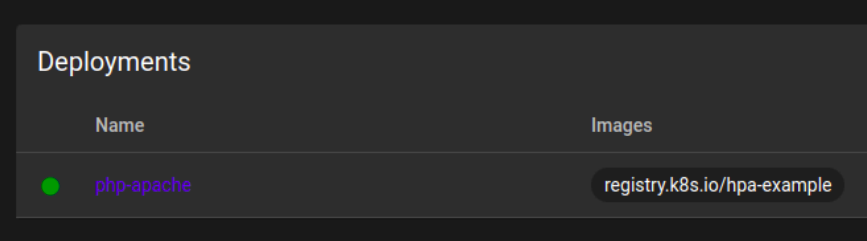
\includegraphics[width=0.45\textwidth]{figures/deployments.png}
  \caption{PHP Apache server deployment.}
  \label{fig:deployments}
\end{figure}

\begin{figure}[!htbp]
  \centering
  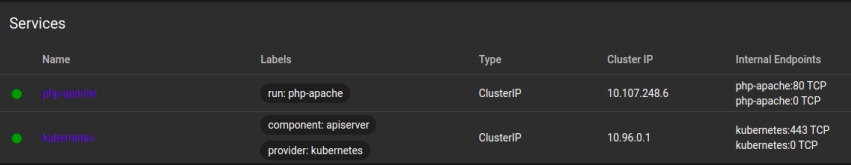
\includegraphics[width=0.45\textwidth]{figures/services.png}
  \caption{PHP Apache server service.}
  \label{fig:services}
\end{figure}

Then, the Horizontal Pod Autoscaler (HPA) is configured to scale the PHP Apache server deployment based on CPU usage.
Then, the load test is executed to increase the CPU usage of the PHP Apache server.
As seen in Figure~\ref{fig:hpa_increasing}, the HPA increases the number of replicas from one to four when the CPU usage exceeds 50\%.
In Figure~\ref{fig:hpa_max}, the HPA reaches the maximum number of replicas, which is six.
Finally, after stopping the load test, the CPU usage decreases, and the HPA decreases the number of replicas from six to one, as shown in Figure~\ref{fig:hpa_decreasing}.

\begin{figure}[!htbp]
  \centering
  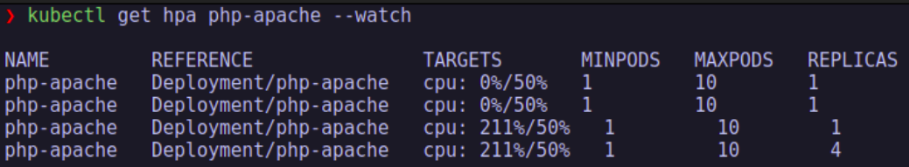
\includegraphics[width=0.45\textwidth]{figures/hpa_increasing.png}
  \caption{HPA increasing the number of replicas.}
  \label{fig:hpa_increasing}
\end{figure}

\begin{figure}[!htbp]
  \centering
  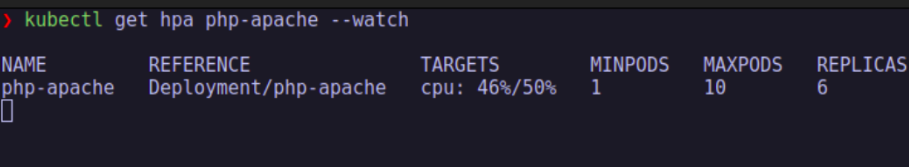
\includegraphics[width=0.45\textwidth]{figures/hpa_max.png}
  \caption{HPA at maximum replicas.}
  \label{fig:hpa_max}
\end{figure}

\begin{figure}[!htbp]
  \centering
  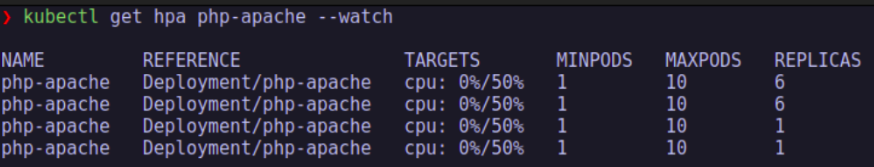
\includegraphics[width=0.45\textwidth]{figures/hpa_decreasing.png}
  \caption{HPA decreasing the number of replicas.}
  \label{fig:hpa_decreasing}
\end{figure}


\subsection{AWS EKS results}

After the execution of the commands to test the autoscaler, as outlined in Listing~\ref{lst:autoscaler-test}, The output of this command is presented in Figure~\ref{fig:metrics}.

\begin{figure}[!htbp]
  \centering
  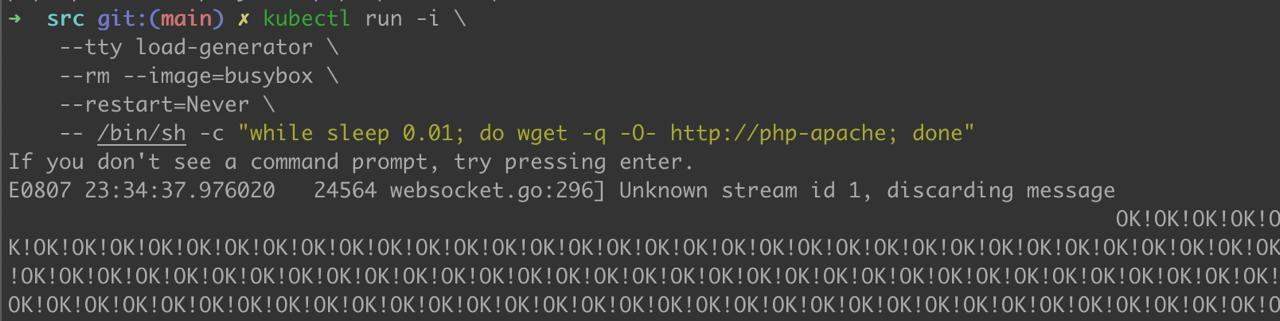
\includegraphics[width=0.45\textwidth]{figures/test-autoscaler.jpeg}
  \caption{Test autoscaler on EKS.}
  \label{fig:test-autoscaler}
\end{figure}

Next, we allowed approximately 2.5 minutes to elapse before proceeding with the command that displays the number of replicas managed by the autoscaler, as shown in Listing~\ref{lst:pods-number}. The output of this command is presented in Figure~\ref{fig:metrics}, where it is evident that nine replicas of the server were generated in response to the load induced by the test command.

\begin{figure}[!htbp]
  \centering
  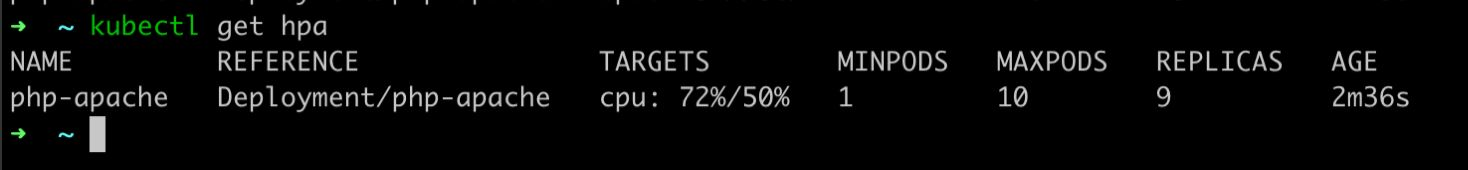
\includegraphics[width=0.45\textwidth]{figures/metrics.jpeg}
  \caption{PHP Apache server metrics.}
  \label{fig:metrics}
\end{figure}
